
\begin{otherlanguage*}{italian}
\chapter*{Sommario}
\addcontentsline{toc}{chapter}{Sommario}
	
	\section*{Introduzione}
	\addcontentsline{toc}{section}{Introduzione}
	Questo documento descrive i principali passi dello sviluppo di un modulo software di computer vision che effettua l'analisi di immagini e comunica i risultati all'architettura cognitiva \mbox{\emph{ACT-R}}\footnote{ACT-R è un'architettura cognitiva, cioè un framework che modella la struttura e il comportamento del cervello umano. Per maggiori informazioni, vedere~\url{act-r.psy.cmu.edu}.}.
	In particolare, il programma ha il compito di riuscire a riconoscere le forme geometriche contenute nelle immagini, i loro colori ed effettuare valutazioni qualitative e quantitative su tali oggetti.

	L'attività è stata svolta presso il \emph{Center for Cognitive Science} dell'università \emph{Albert-Ludwigs-Universität Freiburg} della città di Friburgo.
	Le attività di ricerca del centro, che, come suggerisce il nome, hanno come ambito principale le \emph{scienze cognitive}\footnote{\emph{Le scienze cognitive sono un gruppo di discipline che hanno come scopo lo studio delle capacità cognitive delle menti naturali o artificiali, della possibilità di trasmettere questo sapere agli altri e di averne consapevolezza. La scienza cognitiva è la specifica materia, tra le scienze cognitive, che spiega i modi in cui menti naturali o artificiali filtrano e colgono informazioni percettive, le rielaborano e riescono a intraprendere delle decisioni in base alle circostanze esperite, tanto da "reagire" al mondo esterno anche elaborando degli artefatti}~\cite{legrenzi2005prima}.}, 	
	al momento si focalizzano sul ragionamento spaziale\footnote{Il ragionamento spaziale è una disciplina che si occupa del ragionamento basato sugli oggetti nello spazio; in particolare studia le astrazioni dei concetti spaziali della conoscenza di base sulla quale si basa la prospettiva umana della realtà fisica.} e i ricercatori utilizzano ACT-R come strumento di supporto per i loro studi. 
	
	In questo contesto, il lavoro discusso in questo documento rappresenta una parte del lavoro sviluppato da un team di tre persone, il cui obiettivo ultimo risulta essere quello di migliorare la percezione dell'architettura cognitiva, rendendola più simile a quella umana.  
	Una delle maggiori limitazioni di \mbox{ACT-R}, infatti, è il fatto che esso lavora in un ambiente virtuale, troppo semplice per rappresentare la realtà. 
	Il software sviluppato rappresenta un punto di partenza per permettere ad \mbox{ACT-R} di elaborare oggetti direttamente nel mondo reale, superando tale limite.
	 
	Dal momento che, allo stato attuale, l'architettura cognitiva non presenta dei moduli propri per l'elaborazione dei dati visuali, il software sviluppato è creato come software indipendente. 
	Ciò permette di utilizzare la libreria esterna \mbox{\emph{OpenCV}} per l'elaborazione di immagini e richiede l'introduzione di un protocollo di comunicazione in modo da rendere possibile la comunicazione tra \mbox{ACT-R} e il modulo di visione sviluppato.

	\section*{L'ambiente di lavoro}
	\addcontentsline{toc}{section}{L'ambiente di lavoro}
	L'attività è stata condotta presso il \emph{Center for Cognitive Science} dell'università \emph{Albert-Ludwigs-Universität Freiburg} della città di Friburgo in Germania. 
	Tale centro effettua ricerche scientifiche nell'ambito delle \emph{scienze cognitive}, in particolare studia il \emph{ragionamento spaziale}.

	Le scienze cognitive sono delle discipline che studiano le capacità cognitive della mente, indipendentemente dalla sua natura artificiale o naturale, e spiegano le modalità con cui essa raccoglie e filtra le informazioni percettive ricevute, le rielabora e, sulla base della conoscenza ottenuta, prende delle decisioni che causano poi le reazioni dell'agente agli eventi del mondo esterno. 
	Ciò che viene studiato, in particolare, sono le modalità con cui pensiero, emozione, immaginazione, intelletto e creatività vengono formati~\cite{legrenzi2005prima}.
	La sfida per queste discipline sta nello studiare questi aspetti data l'impossibilità di osservare i processi cognitivi umani nelle diverse fasi in cui essi si sviluppano. 
	
	Un aspetto caratterizzante di tutte le scienze cognitive è la loro natura multidisciplinare: esse infatti accorpano informazioni provenienti da discipline eterogenee (fisiologia, neurologia, intelligenza artificiale, filosofia e psicologia) al fine di creare un modello della mente che sia il più generale possibile~\cite{legrenzi2005prima}. 

	La cognizione spaziale è la scienza cognitiva che studia acquisizione, organizzazione, utilizzo e revisione della conoscenza riguardante gli ambienti spaziali~\cite{r8Cspace}. 
	L'ambito di applicabilità di tale disciplina è molto vasto e comprende sia ambienti reali che modelli astratti e prevede che gli agenti possano essere sia umani che automatici.
	Fondamentale per questa materia è lo studio del processo di ragionamento, che comprende la successione di eventi che portano alla formazione di conoscenza a partire da una serie di premesse. 
	
	Una delle grandi sfide che il centro di ricerca si pone è quella di \emph{gettare le basi per nuove teorie cognitive, riguardanti il ragionamento e la pianificazione, applicando metodi di intelligenza artificiale ed esperimenti comportamentali~\cite{TesiEnr}}.

 

	\section*{Lo stato dell'arte}
	\addcontentsline{toc}{section}{Lo stato dell'arte}
	Di seguito si descrivono i due principali strumenti utilizzati per questo progetto: la libreria di computer vision \emph{\mbox{OpenCV}} e l'architettura cognitiva \mbox{\emph{ACT-R}}.
		
			\subsection*{ACT-R}
			\addcontentsline{toc}{subsection}{ACT-R}
				\mbox{ACT-R} è un'\emph{architettura cognitiva}, cioè l'implementazione di una teoria riguardante il sistema cognitivo umano. Come tale, esso modella struttura e comportamento del cervello umano cercando di spiegare come le diverse componenti collaborino tra loro formando la mente umana.
				
				La teoria di \mbox{ACT-R} si basa sulla \emph{teoria unificata della cognizione} (Unified theory about cognition), sviluppata da John Robert Anderson, docente presso la Carnegie Mellon University. 
				Il concetto fondamentale di tale teoria è che la mente umana si comporti come un sistema integrato.
				Secondo essa, infatti, il cervello è separato in diversi moduli indipendenti, ognuno dei quali è dotato delle proprie funzioni ed è incaricato di svolgere compiti specifici.
				Nel momento di attuare un comportamento, tuttavia, i moduli interagiscono tra loro per raggiungere l'obiettivo comune, proprio come un sistema integrato. 
				La comunicazione tra le diverse parti avverrebbe grazie a specifiche connessioni tra i moduli~\cite{Anderson04anintegrated}.

				Un altro pilastro fondamentale su cui si basa la teoria di \mbox{ACT-R} è la distinzione tra \emph{memoria dichiarativa} e \emph{memoria procedurale}. La prima rappresenta fatti e nozioni che l'essere umano sa ed è conscio di sapere. Per richiamare questo tipo di conoscenza, l'essere umano deve effettuare un processo consapevole. La seconda, invece, si riferisce a tutte quelle abilità e capacità che l'essere umano sa ma che ha imparato in maniera implicita. Esempi di questo secondo tipo di conoscenza sono la lettura e la scrittura~\cite{anderson1976language}. 

				Gli elementi di base dell'architettura di \mbox{ACT-R} sono \emph{chunk} e \emph{produzioni}.
				I chunk rappresentano la memoria dichiarativa e sono delle strutture dati caratterizzate da un tipo, chiamato \emph{type}, e da una lista di coppie, ognuna delle quali è costituita da un attributo, chiamato \emph{slot}, e da un valore, chiamato \emph{value}.
				Le produzioni possono essere paragonate a funzioni e definiscono la sequenza di azioni che possono essere effettuate.
				Ogni produzione presenta un insieme di precondizioni che determinano le condizioni che devono essere verificate affinché la funzione possa essere eseguita ~\cite{actr6refman}.

				Dal punto di vista dell'architettura, \mbox{ACT-R} è organizzato in \emph{moduli}.
				Ciascun modulo è costituito da chunk e da produzioni e svolge un insieme determinato di funzioni cognitive. 
				Essi sono l'analogo dei gruppi di neuroni che si attivano nel cervello nel momento in cui viene effettuata una determinata azione da parte dell'essere umano.
				I moduli sono indipendenti ma possono comunicare tra loro tramite dei \emph{buffer}. 
				La comunicazione, che essenzialmente è uno scambio di chunk, avviene necessariamente in maniera seriale, mentre le operazioni dei diversi moduli possono avvenire in parallelo ~\cite{actr6refman}.
				
				\mbox{ACT-R} è in grado di effettuare infiniti ragionamenti, indipendentemente dal compito da eseguire. 
				Per essere in grado di eseguire una singola attività, tuttavia, necessita di uno specifico \emph{modello}.
				Ciascun modello rispecchia le assunzioni che il creatore di modelli ha riguardo al determinato compito da eseguire.
				Tali assunzioni sono espresse sotto forma di produzioni, che interagiscono con i moduli durante l'esecuzione.
				Questo atto produce una serie di operazioni atomiche cognitive che, passo dopo passo, portano alla soluzione del compito~\cite{Sears2012}. 
				
				Le operazioni presentano delle misure qualitative e quantitative sulla qualità dell'azione stessa, come la correttezza della soluzione trovata e il tempo necessario per completare l'operazione. 
				Ciò conferisce ai modelli la possibilità di predire la sequenza delle azioni cognitive prodotte dagli esseri umani quando questi provano a risolvere un determinato compito. 
				Effettuare dei confronti con le prestazioni degli esseri umani permette di misurare la qualità dei modelli~\cite{Sears2012}.

				Dal punto di vista informatico, \mbox{ACT-R} è scritto in lisp e fornisce una sintassi specifica, simile al lisp, per scrivere i modelli.

			\subsection*{OpenCV}
			\addcontentsline{toc}{subsection}{OpenCV}
				%intro
				\mbox{OpenCV}, acronimo di Open Computer Vision, è una libreria per la computer vision, sviluppata inizialmente da Intel e supportata poi dall'incubatore tecnologico Willow Garage.
				La libreria è multi piattaforma ed è rilasciata sotto una licenza BSD che la rende gratuita e open source. 
				È stata sviluppata per supportare applicazioni in tempo reale e perciò è caratterizzata da una grande efficienza computazionale.
				La versione 2.4 contiene più di 2500 algoritmi, che coprono molte aree della computer vision.

				% computer vision
				La computer vision è essenzialmente la trasformazione di un'immagine o di un video in una nuova rappresentazione, che può essere anche di natura completamente differente rispetto al dato iniziale. 
				L'obiettivo potrebbe essere, ad esempio, una versione in scala di grigi dell'immagine originale, oppure si potrebbe desiderare che il calcolatore sia in grado di prendere una decisione a partire dalle informazioni estratte dall'immagine in ingresso.
				In entrambi i casi si sta parlando di computer vision~\cite{bradski2008learning}.
		
				In generale, la complessità di operazioni di questo tipo risulta essere molto elevata. 
				Ciò che per un essere umano viene percepito come un'attività molto semplice, infatti, può risultare un'operazione molto complessa per un calcolatore, che rappresenta le immagini tramite matrici di numeri. 
				Tale rappresentazione rende complesse molte delle operazioni di visione, comprese quelle più semplici come, per esempio, il riconoscimento di un semplice oggetto.
				Purtroppo al momento questa modalità di descrizione è la migliore alternativa tra le possibilità esistenti~\cite{bradski2008learning}.

				Oltre alla rappresentazione matriciale, uno dei fattori che rendono così complicata la computer vision è la necessità molto frequente di ricostruire un mondo tridimensionale a partire da un'immagine bidimensionale. 
				Questo è un problema mal posto, che ha come diretta conseguenza l'esistenza di infinite soluzioni, cioè infinite ricostruzioni tridimensionali del mondo a partire dall'immagine bidimensionale.
				In particolare, la soluzione dipende dall'angolo con cui si analizza l'immagine~\cite{bradski2008learning}.

				Un fattore che aumenta ulteriormente la complessità dei compiti è la presenza del rumore, che raggruppa tutte le possibili cause di variabilità presenti nel mondo: tempo atmosferico, luminosità, riflessi, movimenti, deformazioni dovute alle lenti o ai sensori e altri fenomeni.
				Il rumore può essere classificato in \emph{noto a priori}, quindi prevedibile, e \emph{non noto a priori}, quindi non prevedibile. 
				Il primo, essendo conosciuto, può essere corretto fino a essere completamente rimosso.
				Questo è il caso, ad esempio, della deformazione delle lenti delle videocamere.
				Il secondo, invece, essendo casuale, non può essere del tutto eliminato ma può essere solamente ridotto.
				Tipicamente si utilizzano metodi statistici per gestire questo secondo tipo di rumore~\cite{bradski2008learning}. 
			 
				Un espediente usato per rendere più facili le operazioni di computer vision è l'introduzione di informazione contestuale. 
				In particolare, più il problema è vincolato, più è facile utilizzare i vincoli per semplificare il problema, più la soluzione ottenuta è affidabile.
				In questo modo, però, la soluzione perde di generalità e diventa specifica per il problema.
				Le tecniche di machine learning, che estraggono automaticamente l'informazione contestuale e la utilizzano per risolvere i problemi, possono essere sfruttate nelle operazioni di computer vision~\cite{bradski2008learning}.
				
				Storicamente, il progetto OpenCV viene avviato nel 1999 da Intel Research, divisione del gruppo Intel dedicata alla ricerca. 
				L'iniziativa è finalizzata a migliorare le applicazioni che richiedono un alto carico di lavoro della CPU, in particolare quelle legate alla visione artificiale. 
				Le intenzioni iniziali comprendono la creazione di codice ottimizzato per un'infrastruttura standard di base per la visione, la diffusione di essa tra gli sviluppatori, la portabilità del codice e la possibilità di creare sia applicazioni di natura commerciale che gratuite grazie all'infrastruttura. 
				Nel 2000 viene rilasciata la prima versione alpha, seguita da cinque versioni beta tra il 2001 e il 2005, che portano nel 2006 a \mbox{OpenCV} 1.0.	
				Nel 2008 l'incubatore tecnologico Willow Garage comincia a supportare il progetto e nel 2009 viene rilasciata la versione 2.0. 
				Come stabilito nel piano di rilascio, ogni sei mesi viene resa pubblica una nuova versione di \mbox{OpenCV}~\cite{OpenCV:ChangeLogs}.

				La libreria mette a disposizione numerose funzioni che coprono diversi rami della computer vision.
				In particolare offre strutture dati per la gestione di immagini e video, funzioni per la visualizzazione e per la gestione degli eventi da parte di tastiera e mouse, procedure per l'interazione con il filesystem, possibilità di manipolare le immagini sia tramite matrici che tramite funzioni di algebra vettoriale, supporto alle strutture dati più comuni e funzioni per tutte le operazioni di base di computer vision: filtraggio, riconoscimento di contorni e di angoli, conversione dei colori, campionamento e interpolazione, operazioni morfologiche e istogrammi.
				Inoltre la libreria integra molte funzioni per l'analisi strutturale dell'immagine, la calibrazione di telecamere, l'analisi del movimento, il riconoscimento di oggetti e il machine learning~\cite{Agam2006}.
				
				Dal punto di vista dei linguaggi di programmazione, la libreria è scritta in C e C++ e presenta interfacce per i linguaggi Python, Java, Ruby e Matlab.
				Dalla versione 2.4 l'architettura è organizzata in moduli, ognuno dei quali svolge specifiche funzioni~\cite{OpenCVDoc}. 
				


	\section*{Gli obiettivi}\label{obiettivi}
	\addcontentsline{toc}{section}{Gli obiettivi}
		%il contesto		
		L'obiettivo ultimo del progetto che comprende questo lavoro è dotare \mbox{ACT-R} di un sistema visivo che sia il più simile possibile a quello umano.
		Per raggiungere tale intento, i ricercatori sono costantemente alla ricerca di tecniche innovative nel campo della visione artificiale che siano il più possibile di uso generale.
		Tal ricerca, tuttavia, non è facile; infatti, la maggior parte delle pubblicazioni riguardanti la computer vision utilizza informazione contestuale, che rende gli algoritmi adatti solamente ai compiti per cui vengono sviluppati.
		
		Questo documento si focalizza solo su un sottoinsieme di funzionalità, cioè quelle che sono state sviluppate dal gruppo di lavoro in cui l'autore di questo documento è stato inserito.	
		Ciò è dovuto al fatto che l'obiettivo dell'intero progetto è molto ambizioso e richiede un tempo ignoto e difficile da stimare a priori. 
		L'autore del documento, invece, è stato inserito per un periodo di tempo limitato in un gruppo di lavoro incaricato di sviluppare soluzioni a problemi specifici, pertanto saranno queste le funzionalità che verranno descritte nei successivi paragrafi.

		%l'obiettivo del team
		L'obiettivo del gruppo di lavoro è quello di creare un software general purpose che riceva in ingresso un flusso video oppure un'immagine ed effettui un processo di riconoscimento di oggetti sui dati in ingresso.
		\mbox{ACT-R} utilizzerà tale software per orientarsi all'interno di un edificio, distinguendo i diversi tipi di stanze a partire dagli oggetti riconosciuti all'interno di ciascuna di esse.

		Come funzionalità fondamentale di tale software, il gruppo deve implementare uno strumento per riconoscere forme geometriche nelle immagini di ingresso. 
		Tali forme rappresentano il punto di partenza per effettuare il processo di riconoscimento degli oggetti. 
		Solo le forme individuate dallo strumento sviluppato, infatti, verranno poi analizzate più in dettaglio per verificare se rappresentino o meno degli oggetti di interesse.

		%l'obiettivo del software
		Un seconda applicazione dello strumento è rendere più facile la definizione del modello al creatore di modelli di \mbox{ACT-R}.
		Per capire meglio questo secondo obiettivo è necessario spiegare come un modello viene creato.
		Il creatore di modelli ha bisogno di un insieme di parametri su cui basare le proprie assunzioni riguardanti le modalità con le quali il cervello umano risolve un determinato compito.
		Tali dati vengono raccolti tramite esperimenti, realizzati grazie a strutture e software appositi, in cui alcuni volontari sono chiamati a risolvere diverse istanze del compito.
		
		Si prenda per esempio l'immagine~\ref{fig:RushHourHumanIta}, che descrive un'istanza del gioco Rush Hour.
		Tale gioco viene utilizzato come test da alcuni psicologi del Centro delle Scienze Cognitive dell'università di Friburgo per confermare alcune ipotesi riguardanti i processi cognitivi umani, la cui spiegazione esula da questo documento.
		L'obiettivo del gioco è spostare le automobili colorate al fine di liberare il percorso tra l'auto rossa e l'uscita, che si trova sulla destra del campo di gioco.
		Ogni automobile, rappresentata da un rettangolo, può spostarsi solo in una direzione, cioè quella parallela al lato più lungo di ciascuna automobile.
		Minore è il numero di spostamenti dell'automobile, migliore è la soluzione. 	

		\begin{figure}[!h]
		  \begin{center} 
			 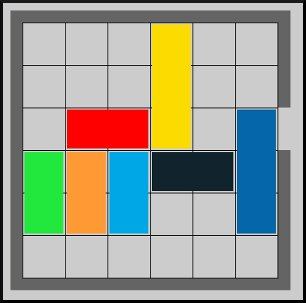
\includegraphics[scale=0.6]{images/ch_03/originale.jpg}	
		  \end{center} 
		  \caption{\textit{Esempio di un istanza del gioco di Rush Hour}}
		  \label{fig:RushHourHumanIta}	
	  	\end{figure}

		Il modello scritto in \mbox{ACT-R} richiede in ingresso la configurazione iniziale di ciascuna delle istanze del problema che si vuole risolvere.
		Al momento, ogni istanza da risolvere, che in \mbox{ACT-R} viene definita tramite una lista di oggetti, deve essere creata manualmente prima della risoluzione. 
		In questo modo, il meccanismo di riconoscimento di \mbox{ACT-R} risulta essere distante da quello umano, il quale riconosce gli oggetti direttamente dall'immagine. 
		Inoltre, dal momento che sia la conferma di un'ipotesi che la stima di determinati parametri richiedono un numero molto alto di istanze, il processo di scrittura manuale comporta una notevole perdita di tempo per i ricercatori.
		Un sistema di riconoscimento automatico, invece, porterebbe una forte innovazione, avvicinando il sistema visuale dell'architettura cognitiva a quello umano, e renderebbe scalabile la creazione di istanze per molti casi di test.
		
		Per ottenere tali obiettivi lo strumento software da sviluppare deve analizzare le immagini che riceve in input, effettuarne l'elaborazione, estraendo l'informazione necessaria alla soluzione dei compiti, salvare tale informazione in una struttura dati dedicata e comunicarla all'architettura cognitiva.
		

	\section*{I Requisiti}
	\addcontentsline{toc}{section}{I Requisiti}	
		Di seguito vengono riportati prima i requisiti funzionali e, successivamente, quelli non funzionali.
			
		\subsection*{Requisiti Funzionali}
		\addcontentsline{toc}{subsection}{Requisiti Funzionali}
			L'obiettivo del lavoro è progettare e implementare un modulo software indipendente, che riceva in input un'immagine e la analizzi estraendo una serie di caratteristiche da essa.
			L'input del software è un'immagine a colori che contiene diverse forme geometriche non sovrapposte. 

			Il software deve riconoscere forme semplici, come:
			\begin{itemize}
	    		\item triangoli;
				\item rettangoli;
				\item quadrilateri;
				\item cerchi.
			\end{itemize}

			Per ciascuna forma, deve calcolare:
			\begin{itemize}
				\item area;
				\item perimetro;
				\item dimensioni;
				\item angolo di rotazione;
				\item una cornice rettangolare, chiamata bounding box;
				\item centro;
			\end{itemize}	
		
			Inoltre, il software deve poter:
			\begin{itemize}
				\item riconoscere il colore di un singolo pixel;
				\item riconoscere il colore di una forma;
				\item calcolare la distanza tra gli oggetti;			
				\item effettuare paragoni dimensionali tra gli oggetti;
				\item calcolare la posizione relativa di un oggetto rispetto a un altro.
			\end{itemize}

			Il software deve essere in grado di comunicare con \mbox{ACT-R}; in particolare, \mbox{ACT-R} deve segnalargli quale deve essere l'immagine da analizzare e richiedere di estrarre le caratteristiche.
			Il modulo, da parte sua, deve ritornare tutta l'informazione estratta ad \mbox{ACT-R}.
		
		\subsection*{Requisiti Non Funzionali}
		\addcontentsline{toc}{subsection}{Requisiti Non Funzionali}
			Per quanto riguarda i \emph{requisiti di prodotto}, il software deve:
			\begin{itemize}
				\item essere multi-purpose;
				\item essere portabile;
			   \item lavorare in background;			
				\item comunicare con \mbox{ACT-R}.			
			\end{itemize}
			
		Per multi-purpose si intende che il software debba essere facilmente modificabile in modo da poter lavorare con gli esperimenti che verranno realizzati in futuro.
		Inoltre, dovrà essere possibile adattare il modulo software al fine di usarlo come riconoscitore di forme per l'orientamento all'interno di un edificio (si veda pagina~\pageref{obiettivi}).
		Al fine di realizzare la comunicazione con \mbox{ACT-R}, i dati devono essere trasmessi in maniera standardizzata.

		Devono, infine, essere rispettati i seguenti requisiti organizzativi:
		\begin{itemize}
				\item il linguaggio dell'implementazione deve essere C++;
				\item la libreria di computer vision utilizzata deve essere \mbox{OpenCV};
			   \item si richiede uno stretto monitoraggio del lavoro.					
			\end{itemize}	

	\section*{Il processo di sviluppo}
	\addcontentsline{toc}{section}{Il processo di sviluppo}
		Di seguito si descrive il framework di sviluppo Scrum, seguito dalle motivazioni che hanno portato all'utilizzo di esso.
		
		\subsection*{Scrum}
		\addcontentsline{toc}{subsection}{Scrum}
			Scrum è un framework per la gestione dei progetti che segue le metodologie agili.
			In quanto tale, esso non definisce in maniera tecnica le modalità che gli sviluppatori devono adottare per ottenere i loro obiettivi ma si concentra sul processo di sviluppo.
			Scrum comprende diverse dimensioni: ruoli, eventi, regole e artefatti; ognuno dei quali è dotato di specifiche funzioni e scopi.
			
			%Ruoli
			Tutti i ruoli del framework sono definiti all'interno dello \emph{Scrum Team}, che è composto da \emph{Product Owner}, \emph{Development Team} e \emph{Scrum Master} e che ha come obiettivo comune aggiungere al prodotto un insieme finito e utilizzabile di nuove funzionalità a intervalli di tempo regolari.
			Il Product Owner rappresenta gli stakeholder\footnote{Con il termine stakeholder si definiscono tutte quelle persone che hanno interesse nello sviluppo del prodotto software.} del prodotto ed è responsabile delle prestazioni del Team.
			Egli definisce i requisiti di ciascuna nuova versione del prodotto e le priorità di ciascuno di essi.
			
			Il Development Team è composto da programmatori e ha il compito di implementare le nuove funzionalità del prodotto.
			Di norma è composto da un numero che va dai tre ai nove membri.
			Caratteristica fondamentale di ogni Development Team è l'auto-organizzazione. 
			Ogni gruppo di sviluppo, infatti, può scegliere il proprio modo di gestire il lavoro e si auto dirige.
			Altra peculiarità è la cross-funzionalità.
			Il Team, infatti, è eterogeneo, cioè contiene al suo interno tutte le competenze necessarie per sviluppare il lavoro e non rischia di essere bloccato da fattori o ruoli esterni ad esso. 
			
			Lo Scrum Master ha il ruolo di verificare che il framework Scrum sia implementato correttamente da tutti i membri dello Scrum Team.
			Egli, in particolare, interagisce con ogni membro del gruppo e lo aiuta a implementare il metodo al meglio, focalizzandosi in particolare sulla minimizzazione delle interruzioni.

			%Eventi
			I due principali obiettivi di tutti gli eventi di Scrum sono controllare l'evoluzione del prodotto nel tempo e minimizzare le interruzioni. 
			Ciò viene realizzato definendo esplicitamente degli intervalli di tempo di durata limitata, in cui le diverse figure professionali aziendali possono incontrarsi per interagire e comunicare tra loro.
			I principali eventi di Scrum sono: \emph{Sprint}, \emph{Sprint Planning Meeting}, \emph{Daily Scrum}, \emph{Sprint Review Meeting} e \emph{Sprint Retrospective Meeting}.

			Lo Sprint è l'intervallo di tempo, la cui durata può variare tra una settimana e un mese, in cui il Team crea una porzione di prodotto completa. 
			Esso inizia con lo Sprint Planning Meeting e termina con Sprint Review Meeting e Sprint Retrospective Meeting.
			
			Lo Sprint Planning Meeting è un evento in cui partecipano tutti i membri dello Scrum Team e rappresenta il momento in cui vengono definite le funzionalità da sviluppare nel prossimo Sprint e le loro priorità.
			Per ciascuna funzione vengono effettuate una stima del tempo necessario per lo sviluppo e una divisione in sotto-attività, ognuna delle quali ha durata massima due giorni.
			Spesso questo incontro è segnato da una progressiva chiarificazione tra Product Owner e Development Team riguardo ai requisiti del prodotto. 
			In questo evento deve anche essere definito lo \emph{Sprint Goal}, cioè uno slogan che riassume l'obiettivo del lavoro dello Sprint e agisce come una sorta di motivazione per tutti i membri del Team.
		
			Il Daily Scrum è un incontro quotidiano della durata di quindici minuti in cui lo Scrum Master incontra il Development Team. 
			In questo evento si valuta il lavoro realizzato e si pianificano le attività della nuova giornata di lavoro.
			Ciascun membro spiega ciò che ha realizzato e cosa farà il giorno successivo.
			Questo incontro permette di misurare la velocità del Development Team e permette ad esso di migliorare le proprie stime per gli Sprint futuri.
			
			Lo Sprint Review Meeting viene realizzato alla fine di ogni Sprint e vi partecipano tutti i membri dello Scrum Team. 
			Durante questa riunione si analizza l'incremento di lavoro effettuato.
			Il Development Team spiega le difficoltà che ha incontrato, come le ha risolte e mostra le nuove funzionalità del prodotto.
			Successivamente si discute di quali funzionalità aggiungere, quali modificare e quali eliminare.

			Durante lo Sprint Retrospective Meeting si analizza l'implementazione di Scrum. 
			In particolare ci si concentra su persone, relazioni, processi e strumenti.
			L'obiettivo è quello di migliorare l'implementazione del framework a ogni Sprint.

			Gli artefatti di Scrum vengono utilizzati per rappresentare il lavoro sotto diversi punti di vista.
			I principali documenti utilizzati sono il \emph{Product Backlog} e lo \emph{Sprint Backlog}.
			
			Il Product Backlog contiene la lista dei requisiti del prodotto, che sono chiamati \emph{Backlog Item}.
			All'interno del Product Backlog i Backlog Item sono ordinati per priorità.
			In generale, gli elementi con priorità maggiore sono quelli più dettagliati, mentre quelli con priorità minore sono  piuttosto generici, in quanto non urgenti e quindi non ancora approfonditi.
			Il documento è dinamico: al termine di ogni Sprint, infatti, le funzionalità che sono state implementate vengono cancellate dal Product Backlog e vengono inseriti i nuovi requisiti o i nuovi dettagli definiti nelle riunioni del Team.

			Lo Sprint Backlog contiene i requisiti da sviluppare nello Sprint corrente, ordinati secondo la priorità stabilita dal Product Owner durante lo Sprint Planning Meeting.
			Ciascun requisito viene diviso in compiti, il cui livello di dettaglio è tale da poter essere misurato giornalmente durante il Daily Scrum.
			Ciascun compito, infatti, deve avere una stima del numero di ore necessarie per essere effettuato, la cui durata non può superare le sedici ore.
			In questo modo, lo Sprint Backlog permette di monitorare l'avanzamento del lavoro ogni giorno dello Sprint.
			Spesso, per rappresentare meglio tale progresso, si utilizza un \emph{Burndown Chart}, che misura il numero completo di compiti completati a partire dall'inizio dello Sprint e paragona l'andamento reale del lavoro con l'andamento ideale con cui esso dovrebbe evolvere~\cite{scrumEnglishGuide}.

			

		\subsection*{Il Processo di Sviluppo Adottato}
		\addcontentsline{toc}{subsection}{Il Processo di Sviluppo Adottato}
			Il Team ha adottato un processo di sviluppo incrementale e iterativo implementando il metodo Scrum.

			Il motivo principale che ha portato a tale scelta è l'alta flessibilità che esso garantisce in caso di cambiamento dei requisiti.
			Spesso, infatti, nei progetti accade che alcune funzionalità, in un primo momento ritenute fondamentali, si rivelino meno importanti di altre, oppure che alcune subiscano cambiamenti, altre vengano eliminate e altre ancora introdotte.
			Le revisioni continue e periodiche previste in Scrum permettono di affrontare in maniera dinamica e flessibile tali modifiche ai requisiti.
	
			Inoltre, l'introduzione di riunioni a intervalli costanti aumenta considerevolmente le prestazioni del gruppo di lavoro.
			Grazie a Scrum, infatti, viene risolto il problema della comunicazione tra le diverse figure professionali che collaborano allo sviluppo del software.  
			Gli stakeholder non hanno più la necessità di chiamare gli sviluppatori in momenti sconvenienti per questi ultimi ma contattano il Product Owner, che riceve i messaggi e li comunica al Development Team durante le riunioni apposite.
			Ciò favorisce il lavoro del Team e dei supervisori, che avviene in un ambiente con minore stress poiché le interruzioni sono minime.

			Un altro vantaggio di Scrum sta nel fatto che il prodotto sviluppato aderisce strettamente ai requisiti definiti.
			Ciò è dovuto agli eventi di durata limitata al termine dei quali vengono presentate le nuove funzionalità e si aggiornano i requisiti.
			Durante gli Sprint Review Meeting il Team mostra le nuove funzionalità ai committenti, che possono dare consigli e chiarire ulteriormente la loro idea riguardo ai compiti che il software deve svolgere.
			Gli eventi di questo tipo sono realizzati appositamente per garantire una stretta aderenza del prodotto ai requisiti.

			Infine, Scrum permette di valutare costantemente le prestazioni del Team.
			Tale valutazione può essere effettuata a diversi livelli da tutti i membri dello Scrum Team.
			Durante lo Sprint Planning Meeting, infatti, si pianifica il lavoro per il prossimo Sprint.
			Nella Sprint Review, si controlla l'effettiva produttività del Team e la si confronta con il piano.
			Su un intervallo temporale più breve, il Daily Scrum è utilizzato per monitorare l'attività giornaliera, mentre il Product Backlog contiene la storia di tutte le modifiche effettuate sul prodotto software sin dalla sua nascita. 
			Grazie a tutti questi eventi e documenti, il progresso del software è costantemente monitorato. 
			
			

	\section*{Il design del software}
	\addcontentsline{toc}{section}{Il design del software}

		% Architettura e processi	
		Dal punto di vista architetturale e dei processi, il sistema è costituito da due moduli indipendenti, l'interprete Lisp che esegue \mbox{ACT-R} e il \emph{Visual Module}, che si occupa di realizzare tutte le funzionalità enunciate nei requisiti.
		I due moduli sono eseguiti da processi diversi, che comunicano tramite il protocollo \mbox{TCP/IP}.
		In particolare, il Visual Module è costituito da due thread, il \emph{Vision Module} e il \emph{Server}.
		Le race condition sono gestite tramite semafori, la libreria \emph{Boost\footnote{Boost è un insieme di librerie per il linguaggio C++ che supportano molte funzionalità, tra cui il multi-threading. Per ulteriori informazioni, vedere il sito ufficiale \url{www.boost.org}}} si occupa di tutte le altre questioni legate al multi-threading.
		
		% Comunicazione
		Il meccanismo di comunicazione utilizzato è sincrono e basato sul protocollo \mbox{TCP/IP}.
		Si è scelto di utilizzare questo protocollo dal momento che è standardizzato, è supportato dagli interpreti Lisp e garantisce flessibilità e scalabilità.
		L'opzione di compilare il software come libreria statica e invocarne le funzioni direttamente, evitando l'introduzione di un protocollo di comunicazione, avrebbe comportato una maggiore efficienza.
		Il problema di questa soluzione è dovuto al fatto che ogni interprete Lisp presenta metodi diversi per gestire le librerie statiche e ciò rende il software non portabile~\cite{SWIGDoc}.

		TCP viene preferito a UDP per le sue caratteristiche di affidabilità e bidirezionalità.
		Inoltre la ridotta quantità di dati contenuta nei messaggi ne rende più opportuno l'utilizzo.
		La comunicazione è sincrona, cioè, una volta effettuata la richiesta, \mbox{ACT-R}, il client, rimane in attesa della risposta del Visual Module, il server. 
		Ciò è coerente con la natura del compito: infatti è desiderabile che l'architettura cognitiva prenda decisioni riguardanti l'ambiente esterno dopo aver ricevuto ed elaborato i dati che lo riguardano.

		Il Modulo Vision Operation è diviso logicamente in tre gruppi di classi: quello che si dedica all'elaborazione di immagini e video, quello che rappresenta le forme riconosciute nelle immagini e quello che gestisce le funzioni di utilità e le eccezioni.
		In figura \ref{fig:classOverviewITA}, si può vedere un diagramma delle classi, realizzato nel linguaggio UML, che descrive ad alto livello i primi due gruppi di classi del Vision Module.
	
		\begin{figure}[h]
		  \begin{center} 
		    \fbox{	
		       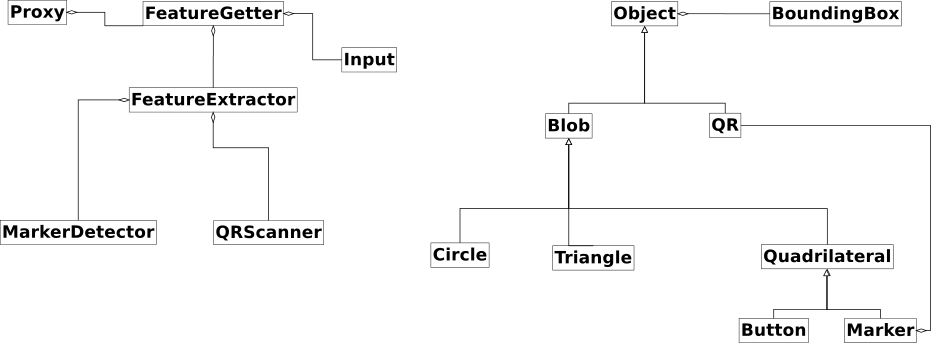
\includegraphics[scale=0.45]{images/ch_05/progettazione_overview.png}
		    }
		  \end{center} 
		  \caption{\textit{Diagramma delle classi che illustra le classi più importanti del Vision Module}}  
		  \label{fig:classOverviewITA}
	 	\end{figure}	
		
		Nel diagramma, sulla sinistra si può vedere l'insieme di classi che elaborano le immagini.
		In particolare, la classe \emph{Feature Extractor} è la classe fondamentale di questo insieme, in quanto effettua tutte le elaborazioni sull'immagine, riconoscendo le forme contenute in essa e creando la corrispondente gerarchia di oggetti. 
		Oltre a tali operazioni, essa riconosce i colori, calcola le distanze tra oggetti, stabilisce le loro posizioni reciproche e li confronta sulla base della dimensione.
		La classe \emph{Input} si occupa di interagire con il filesystem e l'hardware del calcolatore; in particolare, acquisisce immagini e video.
		\emph{Feature Getter} rappresenta un livello di astrazione e offre un'interfaccia semplice a \emph{Proxy}, classe incaricata di preparare i dati in un formato standard per la comunicazione con \mbox{ACT-R}.
		Le classi \emph{MarkerDetector} e \emph{QRScanner} svolgono funzioni non presentate tra i requisiti enunciati in questo documento. Esse acquistano senso se si analizzano gli obiettivi globali del software.
		Le classi sono comunque presenti nel diagramma perché influenzano l'architettura del sistema.

		Sulla destra nel diagramma è presentata la gerarchia degli oggetti.
		\emph{Object} è la super classe e rappresenta qualsiasi oggetto che può essere riconosciuto dal sistema.
		Esso viene specificato dalle due sotto-classi \emph{Blob} e \emph{QR}.
		Blob rappresenta tutte le possibili forme geometriche e la sua presenza ha senso per distinguerle da oggetti di altra natura, come QR o altri che verranno introdotti in futuro.
		QR e \emph{Marker}, esattamente come MarkerDetector e QRScanner, sono oggetti non descritti in questo lavoro ma essenziali per le funzionalità dell'intero sistema.
		Blob viene specializzato dalle classi \emph{Circle}, \emph{Triangle} e \emph{Quadrilateral}, che rappresentano rispettivamente cerchi, triangoli e quadrilateri.
		\emph{Button} rappresenta un bottone e specializza il quadrilatero.



	\section*{Implementazione e testing}
	\addcontentsline{toc}{section}{Implementazione e testing}
		In questa sezione si spiega l'algoritmo utilizzato per il riconoscimento di forme di \emph{n} lati presenti nelle immagini e si discute la strategia di testing applicata.
		
		%implementazione
		L'algoritmo per il riconoscimento di forme è composto da numerosi passaggi.
		Ciò è dovuto alle esigenze di rendere l'operazione il più generica possibile e di ridurre al minimo l'informazione contestuale utilizzata.
		La prima operazione effettuata è un filtraggio, finalizzato alla riduzione del rumore nell'immagine.
		Successivamente, un'operazione di ricerca degli angoli viene applicata ai singoli livelli di colore dell'immagine.
		In particolare, essa viene applicata tre volte per ogni livello: a ogni iterazione vengono utilizzate diverse soglie.
		Il risultato ottenuto è una lista di insiemi di punti; ciascun insieme rappresenta una forma geometrica, la quale è descritta tramite i suoi vertici.
		Per selezionare le figure di \emph{n} lati, dalla lista si estraggono tutti gli insiemi di punti che contengono \emph{n} o più vertici e ciascuno di essi subisce un'operazione finalizzata all'eliminazione dei falsi angoli.
		Può succedere, infatti, che, a causa del rumore presente nell'immagine o di imperfezioni nella procedura di rilevamento degli angoli, vengano individuati più vertici di quelli effettivamente presenti nella forma.
		Un'azione che elimini tali elementi risulta quindi necessaria per il corretto funzionamento dell'algoritmo.
		Al termine dell'operazione, un filtraggio mantiene solo gli insiemi che contengono \emph{n} vertici.
		L'avere applicato l'algoritmo di ricerca degli angoli più volte fa sì che la stessa forma sia riconosciuta più volte.	
		Per questo è necessaria un'altra operazione che elimini le diverse copie della stessa forma, al termine della quale si hanno tutte le forme di \emph{n} lati che sono state identificate nell'immagine. 

		Al momento, l'algoritmo descritto è stato testato solo con triangoli e quadrilateri; tuttavia, può essere facilmente adattato per riconoscere forme che presentano un numero arbitrario di lati. 
		
		%testing
		In questo lavoro, l'obiettivo principale dell'attività di test è quello di valutare correttezza e affidabilità del codice sviluppato.
		A tale fine, il Team ha scelto di applicare una strategia di test che dipendesse strettamente dalla creazione delle classi.
		È stato stabilito, infatti, che la creazione di una suite di test contenente tutti i casi di test di una determinata classe fosse immediatamente successiva alla creazione della classe stessa e che la generazione di tutti i casi di test di un determinato metodo seguisse la creazione del metodo stesso.
		Per garantire una buona copertura dei casi di test, sono state applicate le tecniche del \emph{boundary value} e dell'\emph{equivalent partitioning}.
		Per quanto riguarda il secondo metodo, le due partizioni utilizzate sono state \emph{valori validi} e \emph{valori non validi}.
		Il software utilizzato per la creazione e l'organizzazione di test case e test suite è \emph{CUTE\footnote{Si possono trovare ulteriori informazioni sul software all'indirizzo \url{http://cute-test.com/}}}.
		

	\section*{Conclusioni}
	\addcontentsline{toc}{section}{Conclusioni}
		In questo documento sono descritti i passi principali che hanno portato alla realizzazione di un modulo software in grado di analizzare immagini, estrarre particolari informazioni contenute all'interno di esse e di comunicare tali informazioni all'architettura cognitiva \mbox{ACT-R}, su richiesta di quest'ultima.
		In particolare, le principali informazioni da riconoscere sono	forme geometriche, i loro colori, le loro dimensioni e le loro posizioni.
		Lo scopo ultimo del lavoro di cui il progetto sviluppato fa parte è sviluppare un modulo software per \mbox{ACT-R} finalizzato a rendere la percezione visuale dell'architettura cognitiva più simile a quella umana.

		Il software realizzato utilizza la libreria \mbox{OpenCV} per implementare le operazioni visuali e un metodo di comunicazione basato sul paradigma client-server per lo scambio di messaggi tra il modulo di visione e l'architettura cognitiva. 
		Questa soluzione è semplice, veloce e permette di utilizzare una libreria che offre funzioni sviluppate appositamente per la computer vision.

		Lo strumento implementato riconosce triangoli, quadrilateri e cerchi ed effettua valutazioni qualitative e quantitative riguardo ai colori delle forme, alle loro dimensioni e alle loro posizioni.
		In particolare, esso è utilizzato nell'esperimento Rush Hour per analizzare l'immagine che corrisponde a un'istanza reale di esperimento, creare la lista di oggetti contenuti in essa e comunicarla ad \mbox{ACT-R}.
		In tal modo, l'architettura cognitiva non è obbligata a lavorare su una lista di oggetti, precedentemente creata ad hoc per risolvere la specifica istanza, ma è in grado di elaborare l'immagine direttamente. 
		Questa soluzione conferisce ad \mbox{ACT-R} la possibilità di elaborare oggetti direttamente nel mondo reale.
		%Questa soluzione rende la percezione di \mbox{ACT-R} più simile a quella umana.

		Il numero limitato di funzionalità offerte dal modulo visuale rappresenta il più grande limite dello strumento sviluppato. 
		È sufficiente, tuttavia, aggiungere nuove funzionalità al software per estendere sempre di più l'applicabilità di questa soluzione e usarla in un numero sempre maggiore di casi in congiunzione con \mbox{ACT-R}.

		Al fine di adattare il sistema a lavorare con altri esperimenti, tra le prime funzionalità da introdurre ci sono il riconoscimento di nuovi tipi di forme geometriche, ellissi in particolare, e l'integrazione di uno strumento di \emph{Optical Character Recognition\footnote{Uno strumento di Optical Character Recognition, anche noto come OCR, è un software che riconosce e decodifica lettere e testi nelle immagini.}.}
		Le immagini utilizzate negli esperimenti effettuati dal Centro di Scienze Cognitive, infatti, sono piuttosto semplici: esse contengono forme geometriche elementari colorate uniformemente e, in alcuni casi, del testo.
		L'introduzione di metodi per il riconoscimento di nuove forme e testi renderebbe il sistema più scalabile con la definizione di nuovi esperimenti che richiedono l'elaborazione dell'immagine da parte di \mbox{ACT-R}.

		%L'introduzione di nuove funzionalità, inoltre, potrebbe portare all'applicazione di questo approccio in molti ambiti della ricerca scientifica, incluso nel ragionamento spaziale.
		L'introduzione di nuove funzionalità, inoltre, potrebbe portare grandi miglioramenti nell'ambito della ricerca scientifica, in particolare nel campo delle scienze cognitive.
		Una prima applicazione nell'ambito del ragionamento spaziale arriva direttamente dal Centro di Scienze Cognitive dell'università di Friburgo: il gruppo di lavoro in cui l'autore di questo documento è stato inserito, infatti, ha sviluppato un sistema di navigazione spaziale in ambiente chiuso, basato sull'utilizzo di landmark.
		%Un esempio in questo particolare campo di ricerca viene direttamente dal Centro di Scienze Cognitive dell'università di Friburgo: il gruppo di lavoro in cui l'autore di questo documento è stato inserito, infatti, ha sviluppato un sistema di navigazione spaziale in ambiente chiuso basato sull'utilizzo di landmark.
		Il robot, grazie al modulo di visione sviluppato, infatti, è capace di identificare un landmark, avvicinarvisi, decodificare l'informazione contenuta in esso e inviarla all'architettura cognitiva, la quale, successivamente, comunica al robot come comportarsi sulla base dell'informazione ricevuta.
		Aggiungere, perciò, ulteriori funzioni per il riconoscimento di oggetti aumenterebbe l'applicabilità della soluzione sviluppata.	
		Questo fatto permetterebbe ad \mbox{ACT-R} di svolgere compiti sempre più vari e complessi e ciò potrebbe portare a un numero molto alto di scoperte nell'ambito delle scienze cognitive.


		L'innovazione di questo software consiste nell'aver fornito ad \mbox{ACT-R} la possibilità di elaborare immagini direttamente nel mondo reale.
		Ciò consente di superare uno dei più grandi limiti dell'architettura stessa: lavorare in un ambiente virtuale.
		Spostare la maggior parte dei compiti di visione da \mbox{ACT-R} al modulo di visione porta l'immediato vantaggio di poter utilizzare soluzioni pronte e facili da usare, che consentono di svolgere molti compiti di visione artificiale.
		Inoltre, dal momento che la ricerca in questo campo è molto attiva e produce sempre nuove soluzioni, sarà spesso possibile sperimentare i nuovi algoritmi in nuovi esperimenti.
		Per tutte queste ragioni lo sviluppo di questo software apre la strada a una serie di opportunità per la ricerca nel campo delle scienze cognitive.
	

 
		
\end{otherlanguage*}




